\chapter{Creación del sistema}

El sistema que vamos a crear constara de las siguientes partes. Primero sobre las maquinas con SO Windows se instalara una maquina virtual Ubuntu sobre Virtualbox para trabajar en un entorno linux. A día de hoy existen formas de trabajar directamente con Docker en sistemas Windows tanto por CLI como a través de una interfaz gráfica, aunque estas se basan en emular el kernel de linux. Para este caso se ha optado por trabajar en un entorno linux conocido para hacer más simple el despligue del sistema.

Dentro de dicha máquina Ubuntu se instalará el propio Docker. Mediante Docker crearemos diferentes contenedores. Cada uno de esos contenedores contendrá una imagen de Ubuntu que vendrá con ROS instalado. Estas maquinas se comunicaran entre ellas mediante OpenVPN. Esta red OpenVPN sera configurada en un contenedor diferente, y sera la red a la que el resto de contenedores se conecten.

El esquema del sistema vendría a ser el que se muestra en la Figura \ref{fig:esquemaOriginal}.
\begin{figure}[H] % Con el parámetro H la imagens se muestra justo en el sitio en el que se ha definido
	\centering
	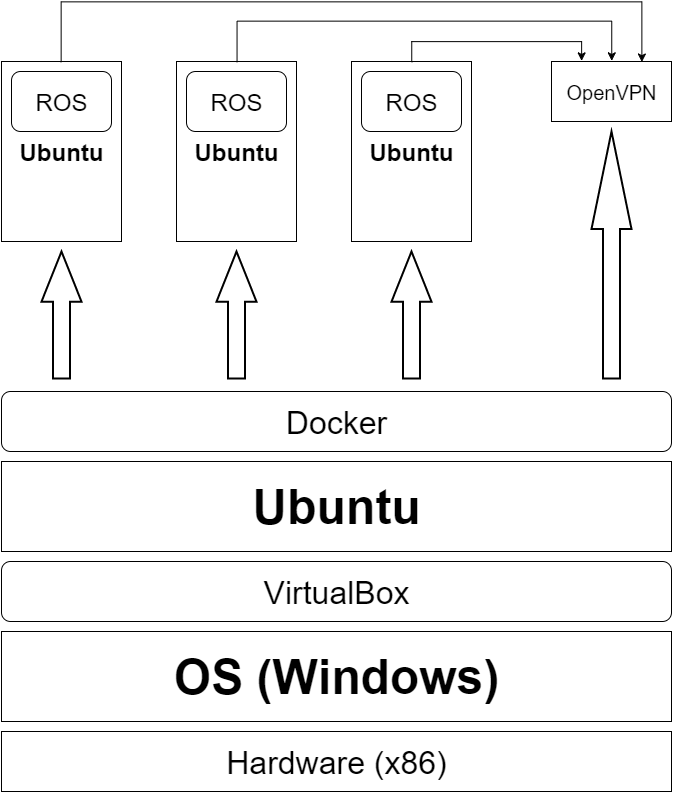
\includegraphics[width=0.8\textwidth]{figuras/esquemaOriginal}
	%		\includesvg{figuras/esquemaOriginal}
	\caption{Esquema del sistema en un ordenador x86}
	\label{fig:esquemaOriginal}
\end{figure}

Posteriormente integraremos nuestro sistema en una Raspberry Pi. El esquema del sistema aplicado en una Raspberry Pi se muestra en la Figura \ref{fig:esquemaRPi}.
\begin{figure}[H]
	\centering
	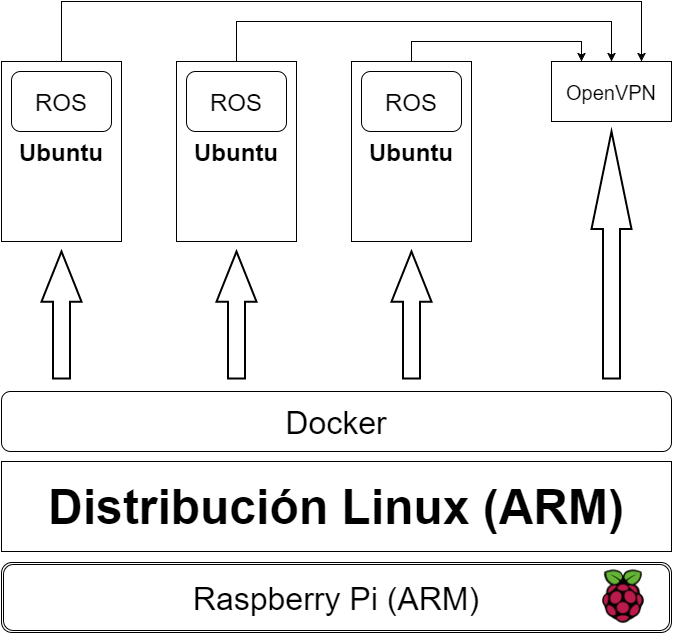
\includegraphics[width=0.8\textwidth]{figuras/esquemaRPi}
	%		\includesvg{figuras/esquemaRPi}
	\caption{Esquema del sistema en una Raspberry Pi}
	\label{fig:esquemaRPi}
\end{figure}

	